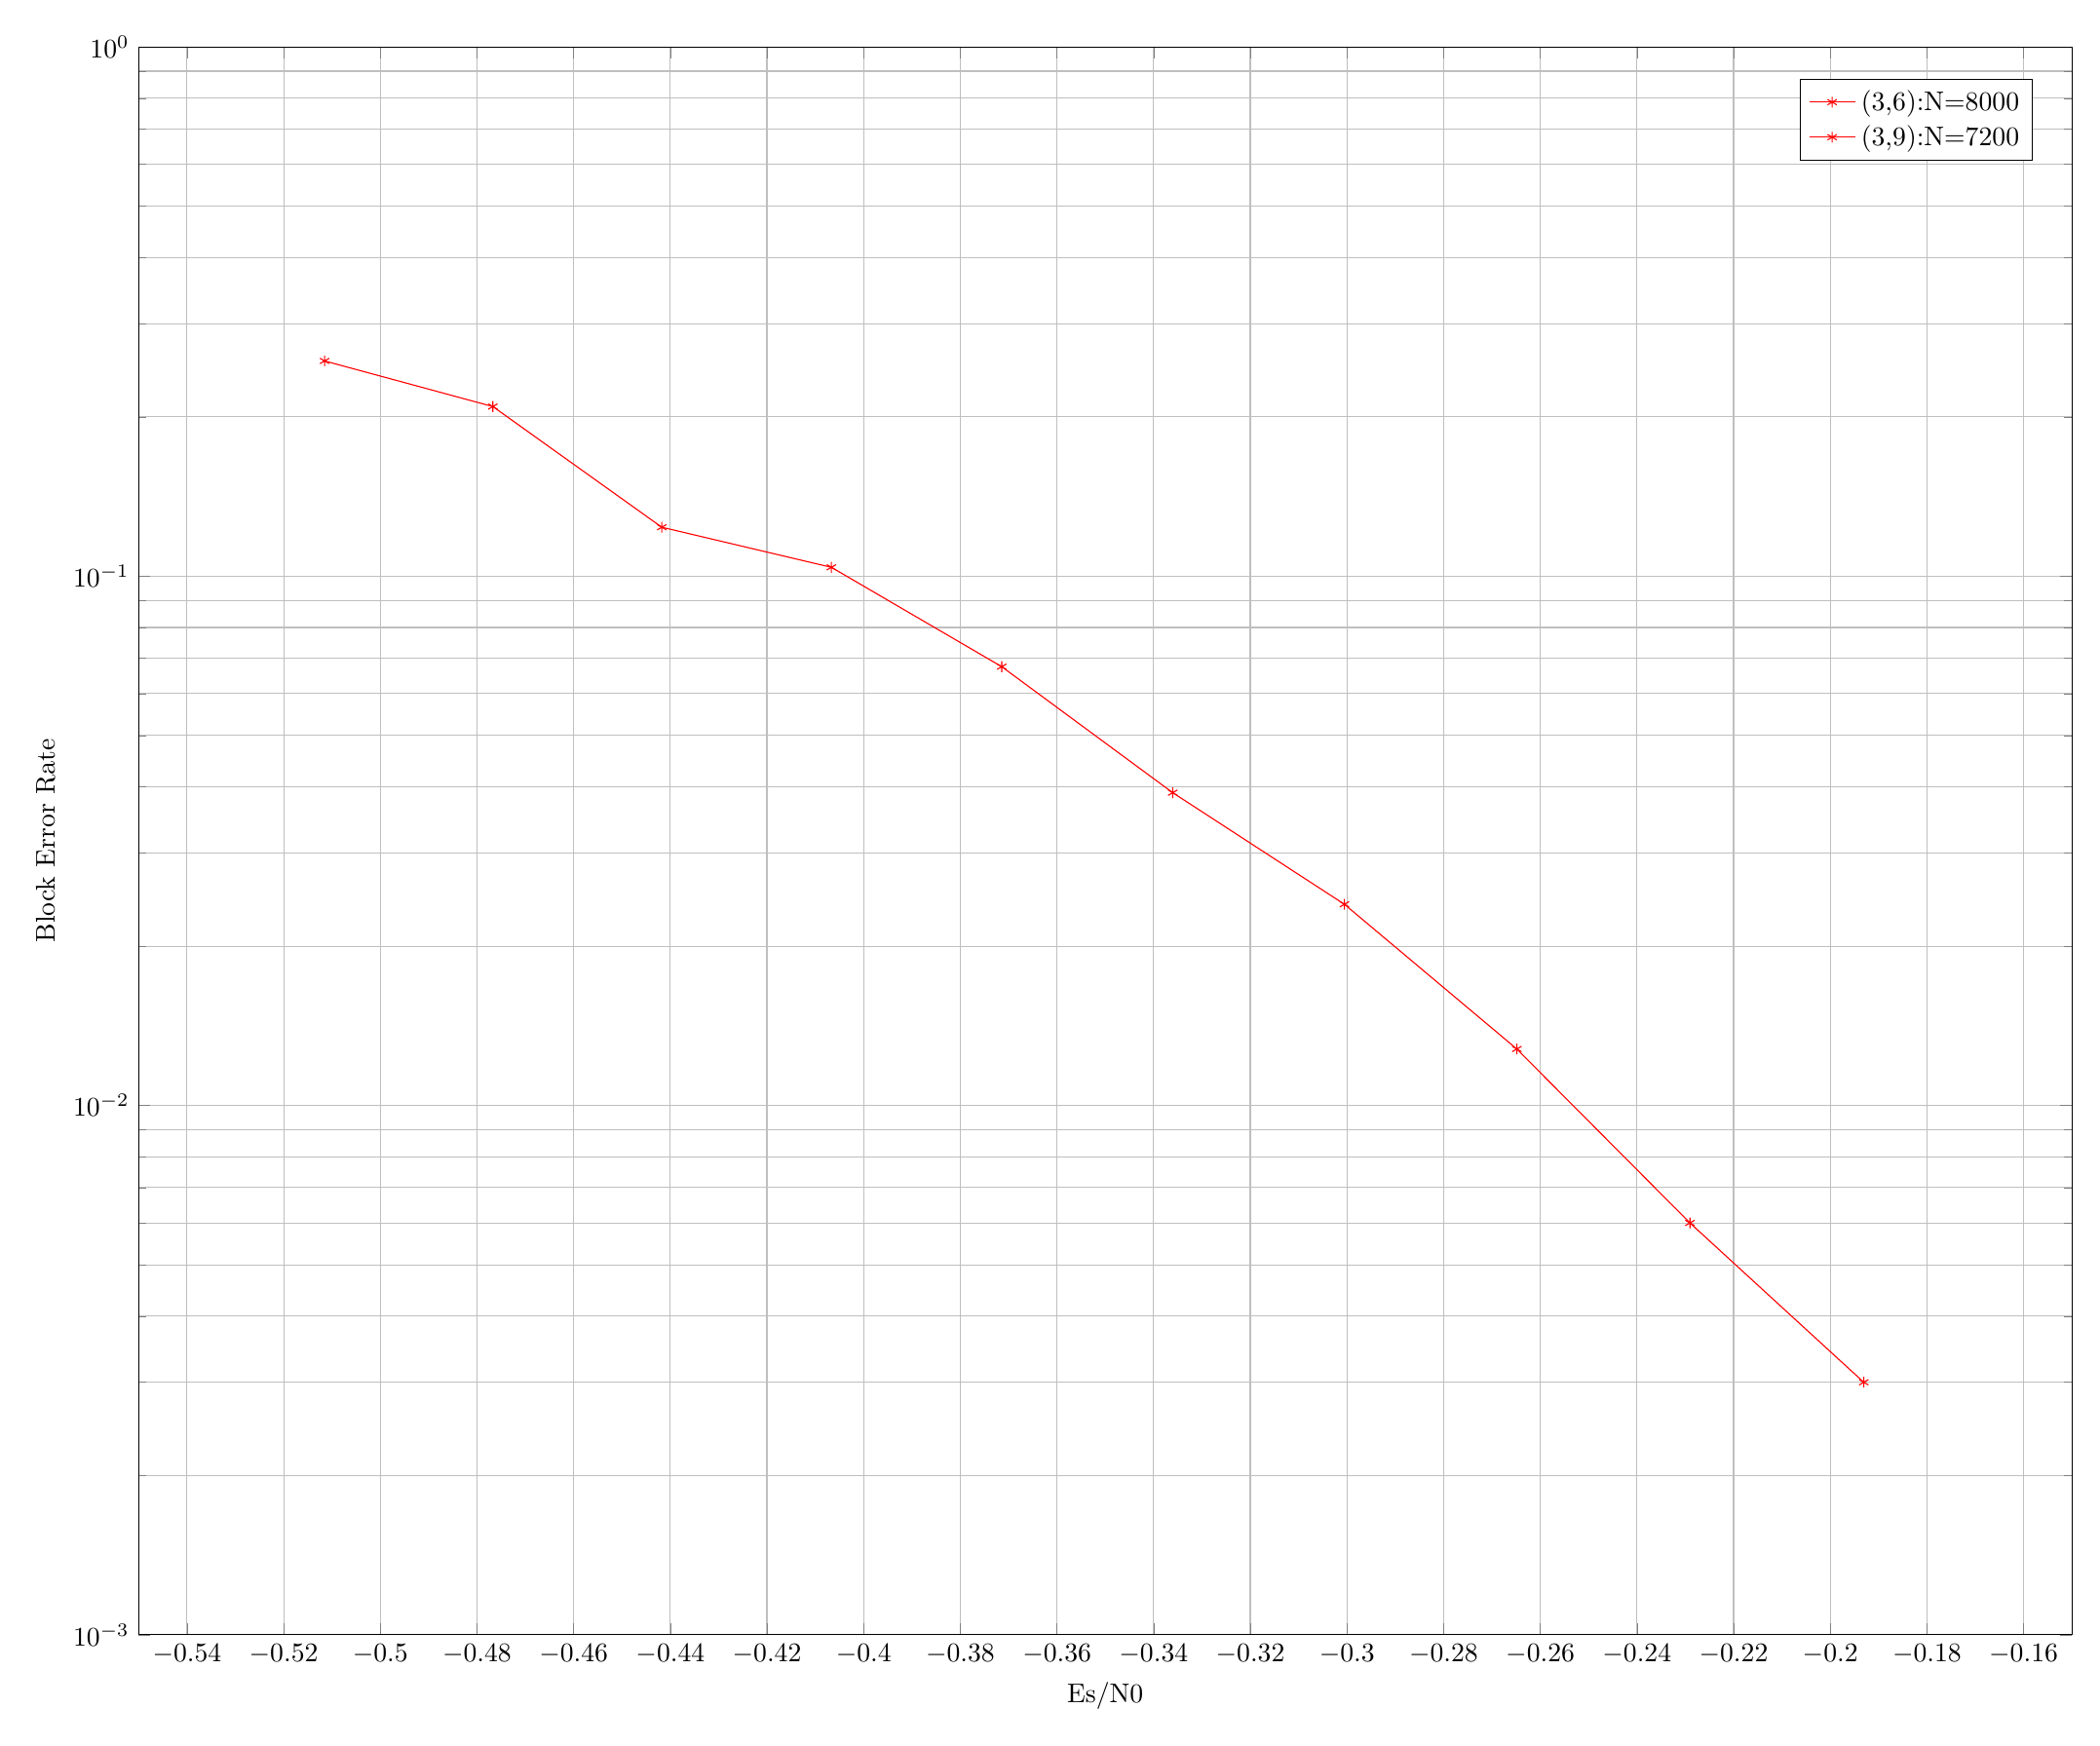
\begin{tikzpicture}
% The SC paramaters for the below set of plots are
% L=16
% w=3.
% So the true rate R is related to design rate R'(=1-dc/dv) as
% 1-R=(L+w-1)*(1-R')/L

\begin{axis}[%
width=9.91942366579178in,
height=8.14846697287839in,
scale only axis,
xmin=-0.55,
xmax=-0.15,
xlabel={Es/N0},
xmajorgrids,
ymode=log,
ymin=0.001,
ymax=1,
yminorticks=true,
ylabel={Block Error Rate},
ymajorgrids,
yminorgrids,
legend style={draw=black,fill=white,legend cell align=left}
]
\addplot [color=red,solid,mark=asterisk,mark options={solid}]
  table[row sep=crcr]{-0.511525224473813	0.255102040816327\\
-0.476711992947787	0.209205020920502\\
-0.441758667557386	0.123762376237624\\
-0.406664116226376	0.103950103950104\\
-0.371427193100643	0.0674763832658569\\
-0.33604673832371	0.039\\
-0.300521577807649	0.024\\
-0.264850522999304	0.0127877237851662\\
-0.229032370641686	0.006\\
-0.193065902530428	0.003\\
};
\addlegendentry{(3,6):N=8000};

\addplot [color=red,solid,mark=asterisk,mark options={solid}]
  table[row sep=crcr]{
   3.0103    0.3738\\
    3.1858    0.2010\\
    3.3649    0.0593\\
    3.5477    0.0220\\
    3.7345    0.0120\\
    3.9254    0.0080\\
    4.1206    0.0040\\
    4.3203    0.0020\\
};
\addlegendentry{(3,9):N=7200};

\end{axis}
\end{tikzpicture}%